\section{Minimum Cost Steiner Trees} \label{sec:5}

\subsection{Minimum Steiner Tree Problem}
Given an (undirected) graph $G = (V, E)$, edge costs $c_e \geq 0$ for all 
$e \in E$, and {\bf terminals} $T \subseteq V$, the goal is to find a 
minimum cost tree that connects all the terminals in $T$. For example, 
the vertices in blue below denote the terminals $T \subseteq V$, 
and the bold edges form a Steiner tree connecting the terminals in $T$. 
\begin{center}
    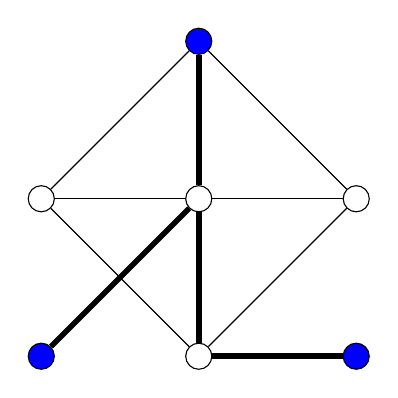
\begin{tikzpicture}[node distance={30mm}, main/.style = {draw, circle}] 
        \node[main, fill=blue] (1) at (2, 4) {}; 
        \node[main] (2) at (0, 2) {};
        \node[main] (3) at (2, 2) {};
        \node[main] (4) at (4, 2) {};
        \node[main, fill=blue] (5) at (0, 0) {};
        \node[main] (6) at (2, 0) {};
        \node[main, fill=blue] (7) at (4, 0) {};

        \draw (1) -- (2);
        \draw[line width=2pt] (1) -- (3);
        \draw (1) -- (4);
        \draw (2) -- (3);
        \draw (2) -- (6);
        \draw (3) -- (4);
        \draw[line width=2pt] (3) -- (5);
        \draw[line width=2pt] (3) -- (6);
        \draw (4) -- (6);
        \draw[line width=2pt] (6) -- (7);
    \end{tikzpicture} 
\end{center}
\vspace{-0.25cm}
Note that we have already seen some particular instances of this problem before.
\begin{itemize}
    \item If $T = \varnothing$, then this problem is trivial; just don't take any edges.
    \item If $|T| = 2$, then this is the shortest path problem.
    \item If $T = V$, then this is the minimum spanning tree problem.
\end{itemize}
However, it turns out that this problem is NP-hard in general!

\subsection{Minimum Metric Steiner Tree Problem} \label{subsec:5.2}
This problem is a minimum Steiner tree problem where we impose the additional 
conditions that
\begin{enumerate}[(a)]
    \item $G = (V, E)$ is complete; and 
    \item $c_{uw} \leq c_{uv} + c_{vw}$ for all distinct $u, v, w \in V$.
\end{enumerate}
Since the edge costs satisfy the triangle inequality, we are living 
in a metric space in some sense, which explains the name of the problem.

It turns out that these problems are equivalent, even though the metric 
version looks like a much more specific case than the original version! 
In our reluctance to call this the \textsc{MST} problem due to minimum 
spanning trees, let's call them \textsc{MSteinerT} and \textsc{MMSteinerT}
respectively. 

If we have an oracle for \textsc{MSteinerT}, then given an instance of 
\textsc{MMSteinerT}, we can simply feed it to the oracle for \textsc{MSteinerT}
as it solves the more general problem. The hard part of the equivalence 
is proving the other direction where if we have an oracle for 
\textsc{MMSteinerT}, then we can also solve \textsc{MSteinerT} efficiently.

Suppose we are given an instance of \textsc{MSteinerT} $(G, c, T)$, 
where $G = (V, E)$. Consider $(G', c', T')$, where
\begin{itemize}
    \item $T' = T$;
    \item $G' = (V, E')$ is the complete graph on the vertices of $G$; and 
    \item $c'_{uv}$ is the length of a shortest $u,v$-path in $G$ with 
    respect to edge costs $c_e$.
\end{itemize}
The following lemma tells us that $(G', c', T')$ is in fact an instance of 
\textsc{MMSteinerT}.

\begin{lemma}{lemma:5.1}
    \begin{enumerate}[(a)]
        \item For every Steiner tree $F$ for the instance 
        $(G, c, T)$, $F' = F$ is also a Steiner tree for the 
        instance $(G', c', T')$ of cost 
        $c'(F') \leq c(F)$. 
        \item For any Steiner tree $F'$ for the instance 
        $(G', c', T')$, there is a Steiner tree $F$ for the 
        instance $(G, c, T)$ such that $c(F) \leq c'(F')$. 
        \item The new edge costs $c'$ satisfy the triangle inequality. In particular, 
        $(G', c', T')$ is an instance of \textsc{MMSteinerT}.
    \end{enumerate}
\end{lemma}\vspace{-0.25cm}
\begin{pf}[Lemma~\ref{lemma:5.1}]
    \begin{enumerate}[(a)]
        \item Since $E' \supseteq E$, we have that $F \subseteq E'$. Moreover, 
        $F$ is still a tree and connects all vertices in $T = T'$. Note that 
        for every edge $e \in E$, we have $c'_e \leq c_e$ because 
        taking the edge $e = uv$ is among one possibility for a $u,v$-path
        and $c'_e$ corresponds to the length of the shortest one. This 
        gives us $c'(F) \leq c(F)$. 
        \item For each $uv \in F'$, consider a shortest $u, v$-path 
        $P_{uv}$ in the original instance $(G, c, T)$. Let 
        \[ K = \bigcup_{uv \in F'} P_{uv} \] 
        be the union of all the edges in these shortest paths. (Note that 
        $K$ is not necessarily a tree.) Since $c(P_{uv}) \leq c'_{uv}$ 
        by construction, we have 
        \[ c(K) \leq c'(F') = \sum_{uv \in F'} c'_{uv}. \]
        Also, $K$ consists only of edges in the original graph $G$ and 
        connects all terminals in $T$. Consider the subgraph  
        with $K$ as the edges and look at the connected component containing 
        the terminals in $T$. Construct a spanning tree $F$ on this connected 
        component. Then $c(F) \leq c(K) \leq c'(F')$ and $F$ connects 
        the terminals in $T$, so it is a Steiner tree for $(G, c, T)$. 
        \item Let $u, v, w \in V$ be distinct. Consider a shortest $u,v$-path 
        $P_1$, a shortest $v,w$-path $P_2$, and a shortest $u,w$-path $P_3$ 
        in $G$ with respect to the original costs $c$. By definition, we have 
        $c'_{uv} = c(P_1)$, $c'_{vw} = c(P_2)$, and $c'_{uw} = c(P_3)$. 
        Note that $P_1$ together with $P_2$ yields a $u,w$-path. Since $P_3$ 
        is a shortest $u,w$-path, it cannot be more expensive than 
        the aforementioned $u,w$-path, so we obtain 
        \[ c'_{uv} + c'_{vw} = c(P_1) + c(P_2) \geq c(P_3) = c'_{uw}, \] 
        so the triangle inequality holds. \qed
    \end{enumerate} 
\end{pf}\vspace{-0.25cm}
Therefore, given an \textsc{MSteinerT} instance, we can efficiently construct 
an \textsc{MMSteinerT} instance. Moreover, if $\textsf{OPT}$ is an optimal solution for 
$(G, c, T)$ and $\textsf{OPT}'$ is an optimal solution for $(G', c', T')$, 
then $c(\textsf{OPT}) \geq c'(\textsf{OPT}')$ by part (a) of Lemma~\ref{lemma:5.1},
and $c'(\textsf{OPT}') \geq c(\textsf{OPT})$ by part (b). This gives us 
$c(\textsf{OPT}) = c'(\textsf{OPT}')$,
so given an oracle to solve \textsc{MMSteinerT}, we can also solve 
\textsc{MSteinerT} instances efficiently by creating a new instance 
of \textsc{MMSteinerT} and feeding it as input to the oracle.

\subsection{An Approximation Algorithm for the Metric Problem} \label{subsec:5.3}
Let's now try to solve \textsc{MMSteinerT} for a given instance $(G', c', T')$;
that is, $G'$ is a complete graph and the costs $c'$ satisfy the triangle 
inequality. Unfortunately, since \textsc{MSteinerT} is NP-hard, so is 
\textsc{MMSteinerT}, because these problems are equivalent! As such, we don't 
know how to solve it efficiently. If there is an efficient algorithm to solve it, this 
shows that $\text{P} = \text{NP}$, resolving the major million dollar problem!

Although we can't find the optimal solution efficiently, we can get an 
approximate solution that isn't too far from optimal in polynomial time. 
Consider the {\bf induced subgraph} of $G'$ on the vertices $T'$, given by 
\[ G'[T'] = (T', \{uv : u, v \in T' \text{ with } u\neq v\}), \] 
which is the complete graph on the vertices in $T'$. The idea is to find a 
minimum spanning tree $F''$ in $G'[T']$ with respect to the costs $c'$. 
We have already seen that this can be done in polynomial time by using 
Prim's algorithm or Kruskal's algorithm. Note that $F''$ is a Steiner 
tree of $(G', c', T')$ of cost $c'(F'')$. 

We cannot hope that $F''$ is an optimal solution in general. For example, 
consider the complete graph $G' = (V', E')$, and let $u \in V'$. Set 
$T' = V' \setminus \{u\}$, and define edge costs by 
\[ c'_{vw} = \begin{cases}
    1, & \text{if } v=u \text{ or } w=u, \\ 
    2, & \text{otherwise.}
\end{cases} \] 
It can be checked that these satisfy the triangle inequality. We illustrate 
this graph below when $|T'| = 3$. 
\begin{center}
    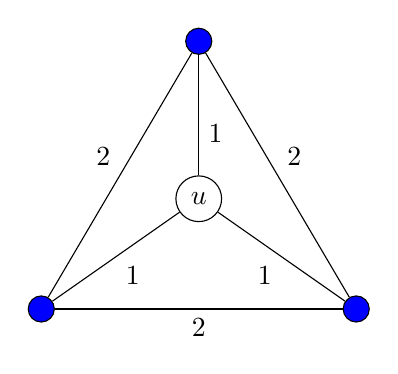
\begin{tikzpicture}[node distance={30mm}, main/.style = {draw, circle}] 
        \node[main] (u) at (0, 0) {$u$}; 
        \node[main, fill=blue] (1) at (0, 2) {};
        \node[main, fill=blue] (2) at (-2, -1.4) {};
        \node[main, fill=blue] (3) at (2, -1.4) {};

        \draw (u) -- (1) node[midway, below right] {1};
        \draw (u) -- (2) node[midway, below right] {1};
        \draw (u) -- (3) node[midway, below left] {1};
        \draw (1) -- (2) node[midway, above left] {2};
        \draw (1) -- (3) node[midway, above right] {2};
        \draw (2) -- (3) node[midway, below] {2};
    \end{tikzpicture} 
\end{center}\vspace{-0.25cm}
For this graph, we see that the optimal solution has value $c(\textsf{OPT}') = 
|T'|$ by taking all the edges with $u$ as an endpoint with cost $1$. 
On the other hand, the induced subgraph $G'[T']$ does not contain $u$, 
so a minimum spanning tree takes only the edges of cost $2$, and there are 
$|T'| - 1$ of them. Therefore, we have 
\[ c'(F'') = 2(|T'| - 1) > |T'| = c(\textsf{OPT}') \] 
when $|T'| \geq 3$, and as $|T'| \to \infty$, we see that 
\[ \frac{c'(F'')}{c'(\textsf{OPT}')} = \frac{2(|T'| - 1)}{|T'|} \to 2. \] 
Fortunately, when using this strategy, this error is the worst it could get.

\begin{lemma}{lemma:5.2}
    Let $F''$ be a minimum spanning tree for $G'[T']$, and let $\textsf{OPT}'$ be 
    an optimal solution for $(G', c', T')$. Then $c'(F'') \leq 2c'(\textsf{OPT}')$.
\end{lemma}\vspace{-0.25cm}
\begin{pf}[Lemma~\ref{lemma:5.2}]
    Let $P$ be an Euler tour on the optimal solution $\textsf{OPT}'$, which is 
    a Steiner tree. That is, $P$ is a path where the starting vertex is 
    the same as the finish vertex, and it visits all the terminals in $T'$.
    Note that $P$ uses every edge in $\textsf{OPT}'$ exactly twice, so 
    $c'(P) = 2c'(\textsf{OPT}')$. Let 
    \[ F^* := \{uv : u, v \in T' \text{ where } u \text{ and } v \text{ 
        are consecutive terminals on the tour $P$}\}. \] 
    Then $F^*$ is a set of edges in $G'[T']$. For every edge $uv \in F^*$, 
    we have by the triangle inequality that 
    \[ c'_{uv} \leq c'(P_{uv}), \] 
    where $P_{uv}$ is the part of the Euler tour 
    $P$ between $u$ and $v$. This gives 
    \[ \sum_{e\in F^*} c'_e \leq c'(P) = 2c'(\textsf{OPT}'). \] 
    Note that $F^*$ connects all the vertices in $G'[T']$ since $P$ connects 
    all the vertices in $T'$. Thus, $G'[T']$ has a spanning tree $\overline{F}$ 
    such that $\overline{F} \subseteq F^*$, so $c'(\overline{F}) \leq 
    2c'(\textsf{OPT}')$. But $F''$ is a minimum spanning tree of $G'[T']$, 
    so we deduce that $c'(F'') \leq c'(\overline{F}) \leq 2c'(\textsf{OPT}')$. \qed
\end{pf}